\begin{figure}
    \centering
    \caption{Visualization of our algorithm for building up stages for the preimage of an interval $(a,b)$ with $-1<a<1<b$}
    \label{fig:sin-a1b-step1}

    \begin{subfigure}{\textwidth}
        \centering
        \caption{stage 0}
        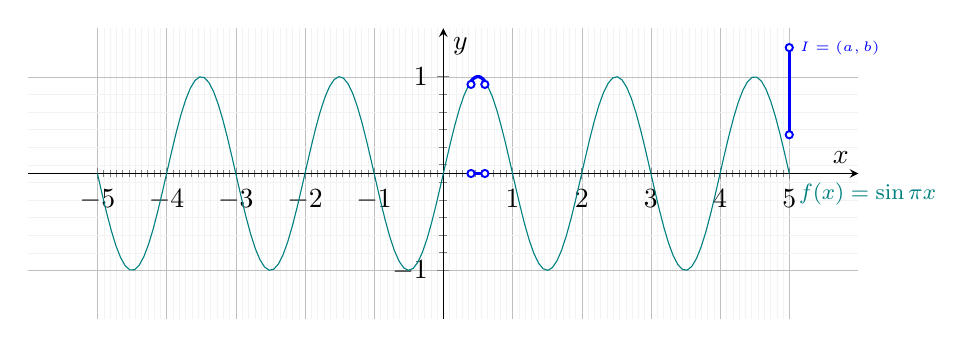
\begin{tikzpicture}
    \begin{axis}[
        width = \textwidth,
        grid=both,
        minor tick num=10,
        grid style={line width=.1pt, draw=gray!10},
        major grid style={line width=.1pt,draw=gray!50},
        axis lines=middle,clip=false,
        height = 150,
        xmin=-6,xmax=6,ymin=-1.5,ymax=1.5,
        ytick={-1,1},
        xtick={-5,-4,-3,-2,-1,0,1,2,3,4,5},
        xticklabels={$-5$,$-4$, $-3$,$-2$,$-1$,$0$,$1$,$2$,$3$, $4$, $5$},
        xticklabel style={black},
        xlabel=$x$,
        ylabel=$y$
    ]
    \draw[very thick, blue] (axis cs:5,0.4) -- (axis cs:5,1.3) node[right, font=\tiny] {$I=(a,b)$};
    \fill [color=white,draw=blue,line width=0.7pt] (axis cs:5,0.4) circle (1.3pt);
    \fill [color=white,draw=blue,line width=0.7pt] (axis cs:5,1.3) circle (1.3pt);


    \addplot[domain=-5:5,samples=150,teal]{sin(deg(pi*x))} node[below right,pos=1,font=\footnotesize]{$f(x)=\sin \pi x$};

    \addplot[domain=.4:0.6,samples=100, very thick,blue]
    {0} node[below right,pos=1,font=\footnotesize]{};
    
    \addplot[domain=.4:0.6,samples=100, very thick,blue]
        {sin(deg(pi*x))} node[below right,pos=1,font=\footnotesize]{};
    \fill[color=white,draw=blue,line width=0.7pt] (axis cs:0.4,0.92) circle (1.3pt);
    \fill[color=white,draw=blue,line width=0.7pt] (axis cs:0.6,0.92) circle (1.3pt);
    \fill[color=white,draw=blue,line width=0.7pt] (axis cs:0.6,0) circle (1.3pt);
    \fill[color=white,draw=blue,line width=0.7pt] (axis cs:0.4  ,0) circle (1.3pt);

    \end{axis}
  \end{tikzpicture}
    \end{subfigure}
    \begin{subfigure}{\textwidth}
        \centering
        \caption{stage 1}
        \input{images/4/sin-a1b-step2}
    \end{subfigure}
    \begin{subfigure}{\textwidth}
        \centering
        \caption{stage 2}
        \input{images/4/sin-a1b-step3}
    \end{subfigure}

\end{figure}